\documentclass{article}
\usepackage{graphicx}
\usepackage[utf8]{inputenc}
\usepackage[english,greek]{babel}
\usepackage{float} % Required for H placement specifier
\usepackage{geometry} %Για να προσαρμώσω το  margin της σελλίδας.
\usepackage{ragged2e} %Για πλήρης στίχηση.
\usepackage{caption}

\geometry{left = 1in, right = 1in, top= 1in, bottom = 1in}

\setlength{\parindent}{1em}

\begin{document}

\begin{center}
    \vspace*{-2cm} % Adjust the value as needed
    \centering
    \hspace*{-0.1cm} % Adjust the value to move the image more towards the left
    
\includegraphics[width=1\textwidth]{Images/Lab_Title.png} % Adjust width as neededfilename of your images
\end{center}

\vspace{1cm}

% Title
\centering
{ \large \bfseries Αναφορά Εργαστηριακής Άσκσησης 0} % title of the report

\vspace{0.5cm}

% add your name here
Αριθμός Ομάδας:66\\

\raggedright
Λαμπράκης Μιχάλης   \hspace{2em}        2020030077\\
Δήμας Χρήστος       \hspace{3.8em}      2021030183\\

\vspace{1cm}

{ \large \bfseries 1.Σκοπός της Άσκησης}\\ % title 1

\begin{justify}
\hspace{1.5em}
Ο σκοπός της Άσκησης είναι η εξοικείωση με το εργαλείο 
\selectlanguage{english}
Xillinx Core Generator
\selectlanguage{greek}
καθώς και η μοντελοποίηση και η υλοποίηση μιας μονάδας μνήμης με δυνατότητα εγγραφής και ανάγνωσης \selectlanguage{english}16-bit \selectlanguage{greek}αριθμών.

\end{justify}

\vspace{0.5cm}

{ \large \bfseries 2.Περιγραφή της Σχεδίασης}\\ % title 2

\begin{justify}
\hspace{1.5em}
Αρχικά το πρώτο βήμα της σχεδίασης ήταν να σχεδιαστεί \selectlanguage{english} State Diagram \selectlanguage{greek}για την \selectlanguage{english}FSM\selectlanguage{greek} (η οποία έχει τον ρόλο του \selectlanguage{english}Memory Controller\selectlanguage{greek}).
Πέρα από τις δοσμένες εισόδους προσθέσαμε και το \selectlanguage{english}Write Enable\selectlanguage{greek}, μεταβλητή η οποία παίρνει την τιμή '1' στις καταστάσεις \selectlanguage{english}Writing\selectlanguage{greek} και \selectlanguage{english}Read/Write\selectlanguage{greek} (όταν δηλαδή επιτρέπται το γράψιμο).

\end{justify}

\vspace{0.5cm}

% \begin{center}
% % \begin{figure}
%     % \centering
%     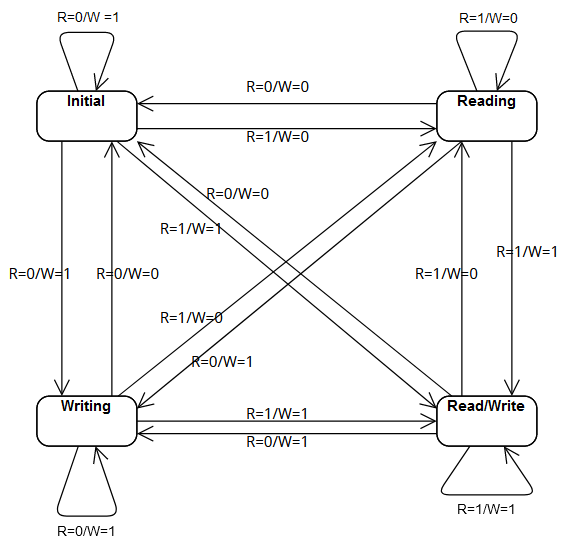
\includegraphics[width=0.6\textwidth]{Images/state_diagram.png} % Adjust width as neededfilename of your images
%     \captionsetup{font=footnotesize} % Set caption font size to small
%     \captionof{figure}{\selectlanguage{english}State Diagram\selectlanguage{greek} του \selectlanguage{english}Memory Controller\selectlanguage{greek}}
%     \label{fig:scehmatic}
% % \end{figure}
% \end{center}

\begin{minipage}[t]{0.4\textwidth}
        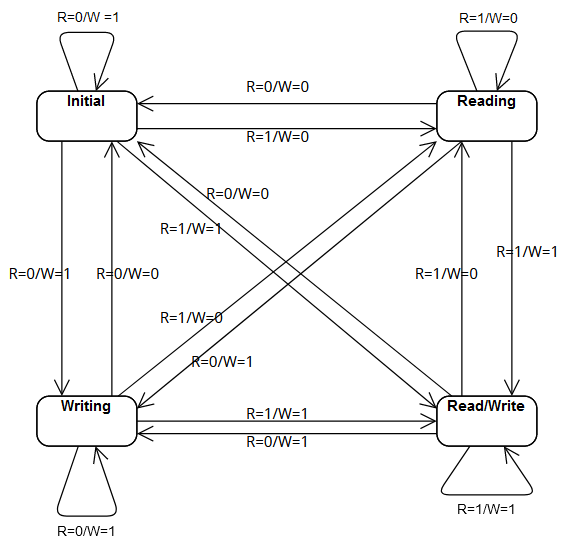
\includegraphics[width=\textwidth]{Images/state_diagram.png}
        \captionsetup{font=footnotesize} % Set caption font size to small
        \captionof{figure}{\selectlanguage{english}State Diagram\selectlanguage{greek} της \selectlanguage{english}FSM\selectlanguage{greek}}
        \label{fig:scehmatic}
\end{minipage}
\hfill
\begin{minipage}[t]{0.55\textwidth}
        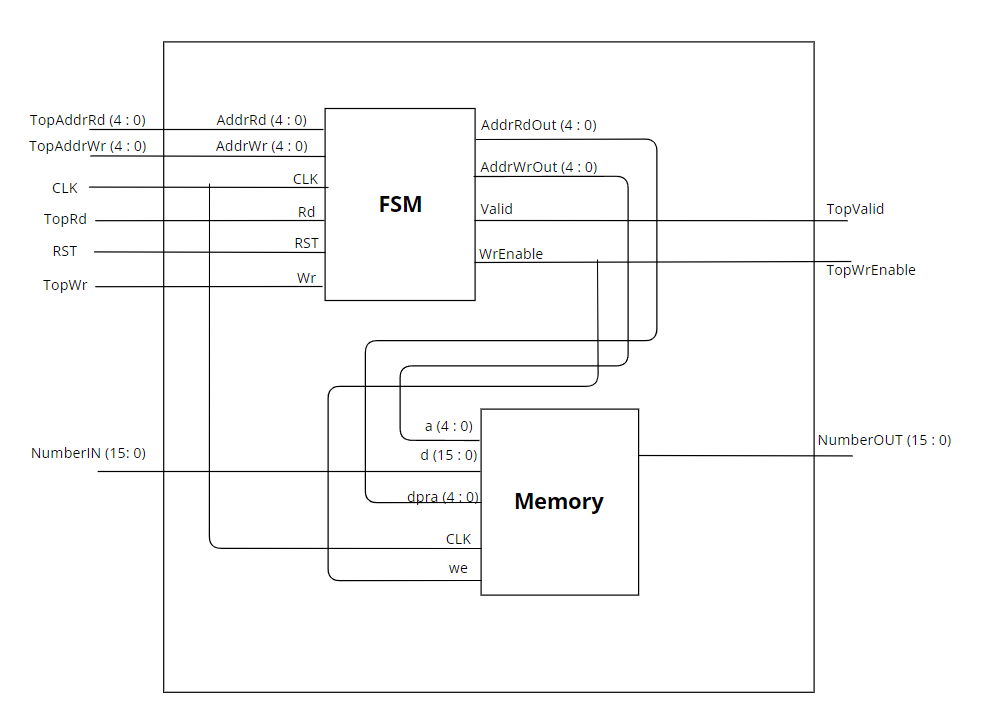
\includegraphics[width=\textwidth]{Images/image.png} % Provide the filename of your second image
        \captionsetup{font=footnotesize} % Set caption font size to small
        \captionof{figure}{\selectlanguage{english}Block Diagram\selectlanguage{greek}}
        \label{fig:second_image}
\end{minipage}

\newpage

\begin{justify}
\hspace{1.5em}
Επιπλέον, για την επίτευξη συγχρονισμού των σημάτων \selectlanguage{english}Write\selectlanguage{greek} με \selectlanguage{english}Write Enable\selectlanguage{greek} και \selectlanguage{english}Read\selectlanguage{greek} με \selectlanguage{english}Valid\selectlanguage{greek} κάναμε την \selectlanguage{english}FSM\selectlanguage{greek} να λειτουργεί σε \selectlanguage{english}falling edge\selectlanguage{greek}. Παρατηρήθηκε οτι διαφορετικά υπήρχε μια μια μικρή καθυστέρηση μεταξύ των σημάτων. Για την δημιουργία της μνήμης επιλέγχθηκε \selectlanguage{english}Distributed Dual-Port RAM\selectlanguage{greek}. Τέλος η σύνδεση των δύο επιμέρους υποσυστημάτων( μνήμης και \selectlanguage{english}FSM\selectlanguage{greek} ) γίνεται στο αρχείο \selectlanguage{english}TopLevel.vhd\selectlanguage{greek} με βάση το \selectlanguage{english}Block Diagram\selectlanguage{greek} (Σχήμα 2).
\end{justify}

\vspace{0.5cm}

{ \large \bfseries 3.Αναφορά Αποτελεσμάτων-Επιβεβαίωση Λειτουργίας}\\ % title 3

\begin{justify}
\hspace{1.5em}
Η επιβεβαίωση λειτουργίας του συστήματος έγινε με \selectlanguage{english}Test Bench\selectlanguage{greek}, 16 στο σύνολο, για όλες τις πιθανές καταστάσεις (4 καταστάσεις και 4 περιπτώσεις για την κάθε κατάσταση άρα 16 πιθανές περιπτώσεις).
\end{justify}

\begin{center}
    \centering
    \hspace*{-1.8cm} % Adjust the value to move the image more towards the left
    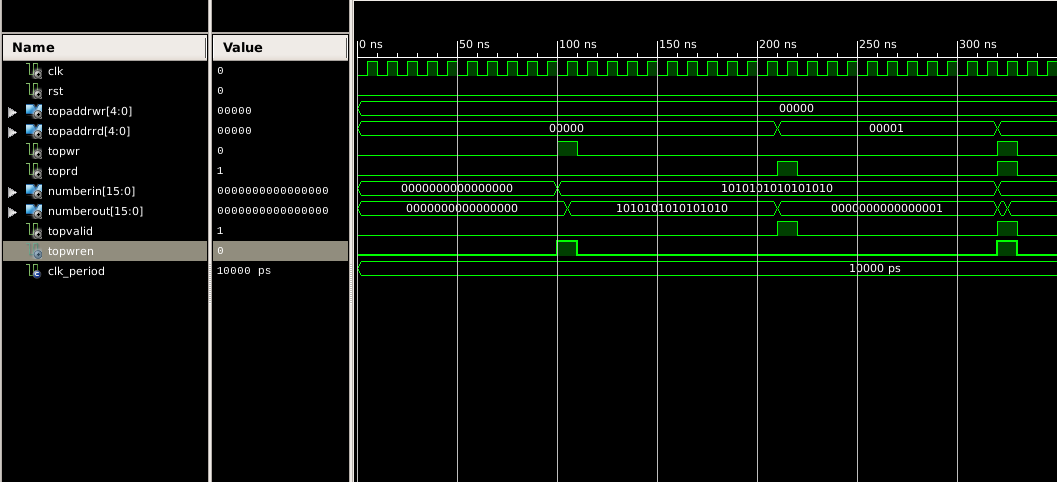
\includegraphics[width=1.2\textwidth]{Images/Screenshot_1.png} % Adjust width as neededfilename of your images
    \captionsetup{font=footnotesize} % Set caption font size to small
    \captionof{figure}{Αποτελέσματα Προσομοίωσης}
    \label{fig:third_image}
\end{center}

\vspace{0.5cm}
\begin{justify}
\hspace{1.5em}
Αρχικά στο Σχήμα 3 το σύστημα βρίσκεται στην αρχική κατάσταση. Το \selectlanguage{english}Write\selectlanguage{greek} γίνεται '1' και δίνεται μια είσοδος για εγγραφή στην μνήμη. Παρατηρούμε ότι το \selectlanguage{english}WriteEnable\selectlanguage{greek} γίνεται '1'. Έπειτα το \selectlanguage{english}Write\selectlanguage{greek} γίνεται '0' και το σύστημα επιστρέφει στην αρχική κατάσταση. Στη συνέχεια το Έπειτα το \selectlanguage{english} Read\selectlanguage{greek} γίνεται '1' και δίνεται διεύθυνση μνήμης για ανάγνωση όπου και εμφανίζεται η εγγεγραμένη στην μνήμη τιμή και το σήμα Valid γίνεται '1'. Αντίστοιχα επιστρέφουμε στην αρχική κατάσταση. Τέλος με είσοδο \selectlanguage{english}Read = 1\selectlanguage{greek} και \selectlanguage{english}Write = 1\selectlanguage{greek} το σύστημα περνάει στην τρίτη κατάσταση όπου πρώτα γίνεται η ανάγνωση και μετά η εγγραφή στη θέση της μνήμης. Με τον ίδιο τρόπο έχουν γίνεται \selectlanguage{english}Test\selectlanguage{greek} για όλες τις πιθανές καταστάσεις.
    
\end{justify}

\vspace{0.5cm}

{ \large \bfseries 4.Συμπεράσματα}\\ % title 3
\begin{justify}
Η άσκηση αυτή μας φαίρνει πρώτη φόρα σε επαφή με το εργαλείο \selectlanguage{english}Xillinx Core Generator\selectlanguage{greek} και τον έλεγο μνήμης στη \selectlanguage{english}VHDL\selectlanguage{greek}. Το σύστημα λειτουργεί σωστά σε όλες τις πιθανές περιπτώσεις πράγμα που επιβεβαιώνεται από τα \selectlanguage{english}Test Bench\selectlanguage{greek}.

\end{justify}

\end{document}